\section{Design Requirements \& Hardware Implementation} \label{sec:hardware}\label{sec:design_requirements}

\subsection{Purpose}
Electronics gain calibration of the \wcd, \lsv\ and \tpc\ is done with dedicated Laser systems, that are in place in each of the three subdetectors. The Laser calibration in the \wcd\ is sufficient to veto muons (and their secondaries) with high efficiency \cite{veto_paper}. The \tpc\ detector response has been calibrated using the internal ${39}$Ar as well as $83m$Kr, that has been added into the \lar\ recirculation system during dedicated calibration campaigns \cite{DS:firstpaper}.

The goal with the CALibration source Insertion System (CALIS) is to study and calibrate the detector response of the \tpc\ and the \lsv\ as well as the detection efficiency of internal neutrons interacting in the \tpc\ and \lsv\ using radioactive gamma and neutron sources. This complements and extends the physics reach of internal source and Laser calibration. 

The center of the \lsv\ is about 6 m below the gate valve inside CRH
%=6145=70+120+400+3455+20+251+1372+457 from http://darkside-docdb.fnal.gov:8080/cgi-bin/RetrieveFile?docid=858&filename=NoFlyZone-DS50_vers02.pdf&version=14
 and the $6''$ wide organ pipes are vertical, yet about 80 cm off center in the XY plane as shown in Fig.~\ref{fig:CALIS_photos}. For \tpc\ calibration the radioactive source has to be positioned in immediate contact with the cryostat, in order to minimize rate losses through absorption in particular for low energy sources such as $^{57}$Co (122 keV). 

\subsection{Deployment \& Articulation Mechanism}\label{sec:DeploymentArticulation}
%focus on the mechanism --- protection provided by the housing is discussed below:
This requirement precludes a single cable solution deployed from within a glove box as has been used in several scintillator experiments \cite{KamLAND-MiniCal, DayaBay_zaxis}. Instead the apparatus consists of the housing, which has been installed in CRH (Fig.~\ref{fig:CALIS_photos}, left) and the deployment device is attached to the housing through two stainless steel cables that are wound up on cable spools and allow the lowering of the device into the \lsv, next to the cryostat (Fig.~\ref{fig:CALIS_photos}, right).
\mymarginpar{in fig.\ref{fig:sourceArmRotation} the drawing should show the arm articulate towards the left, since when the left spool is engaged, the arm articulates towards the left.}
\begin{figure}[htbp]
 \centering
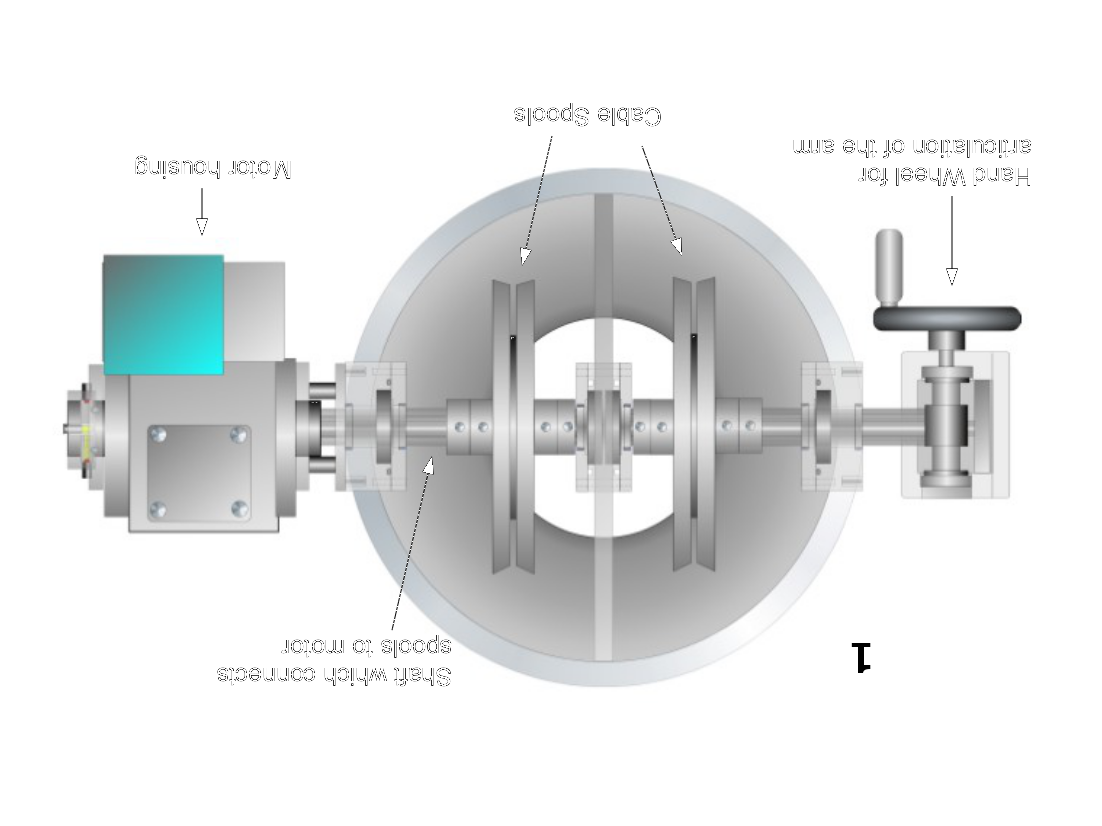
\includegraphics[width=0.9\textwidth]{Figures/gearDrawing}
  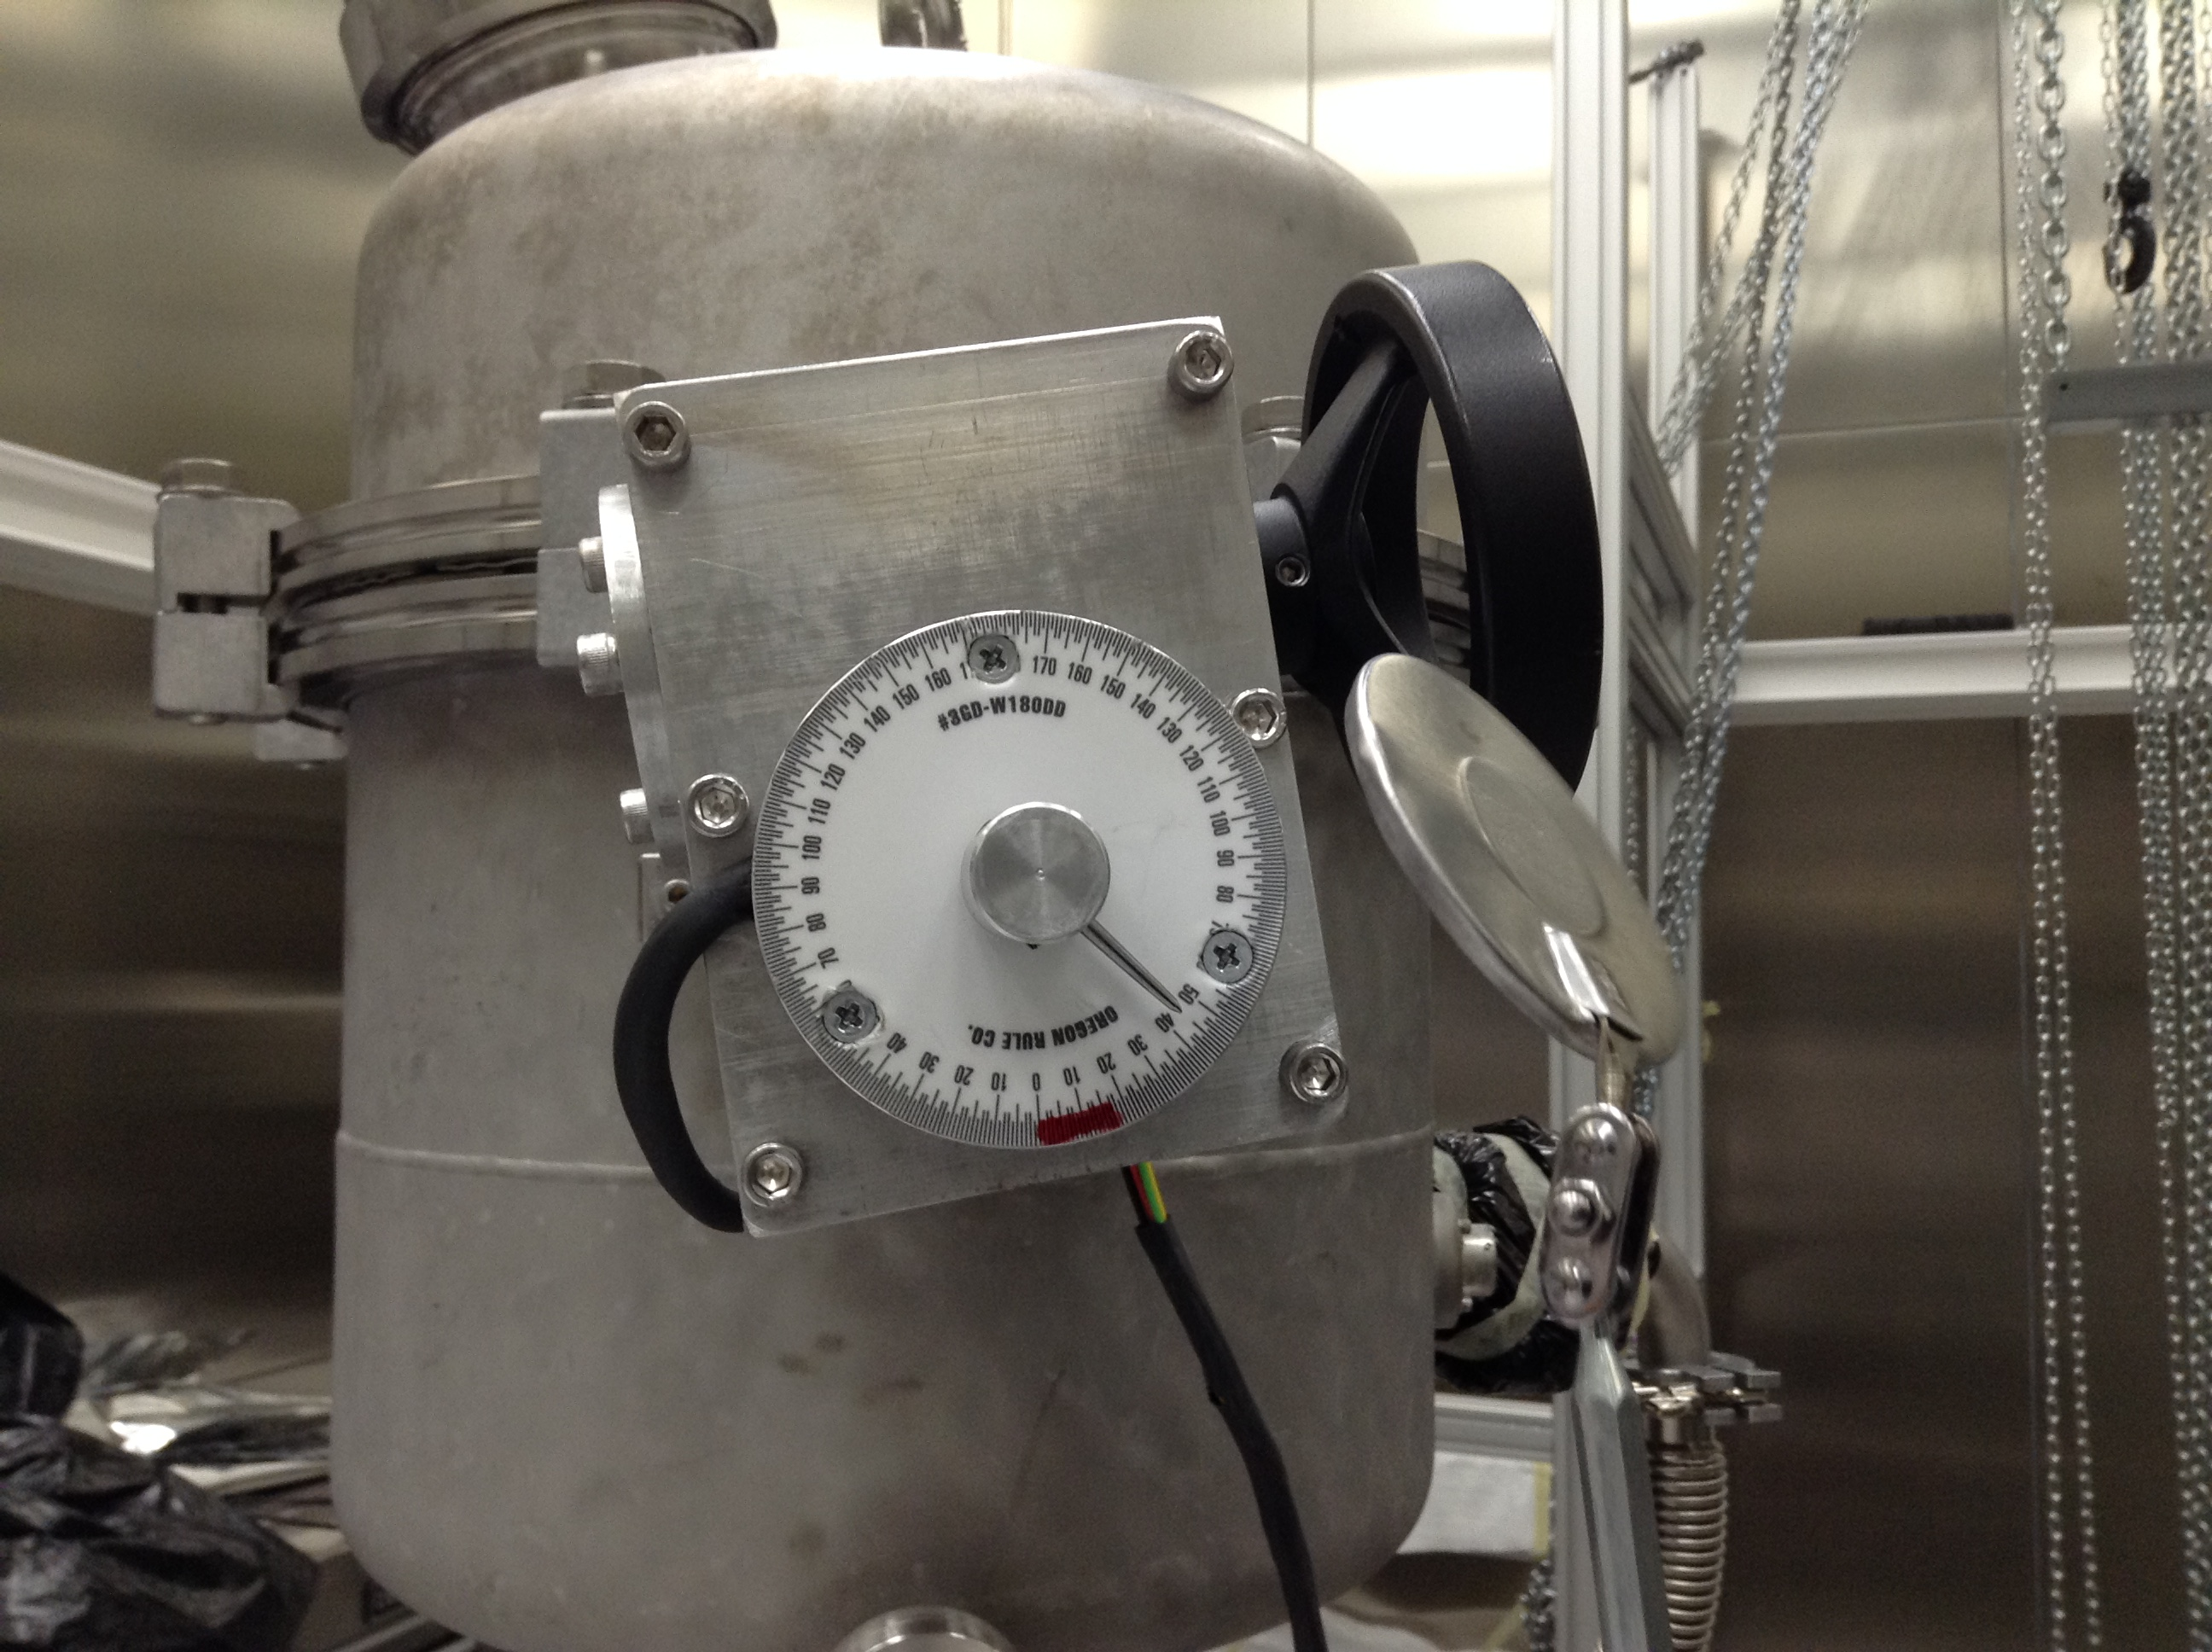
\includegraphics[width=0.48\textwidth]{Figures/ArticulationProtractor_IMG_2667.JPG}
  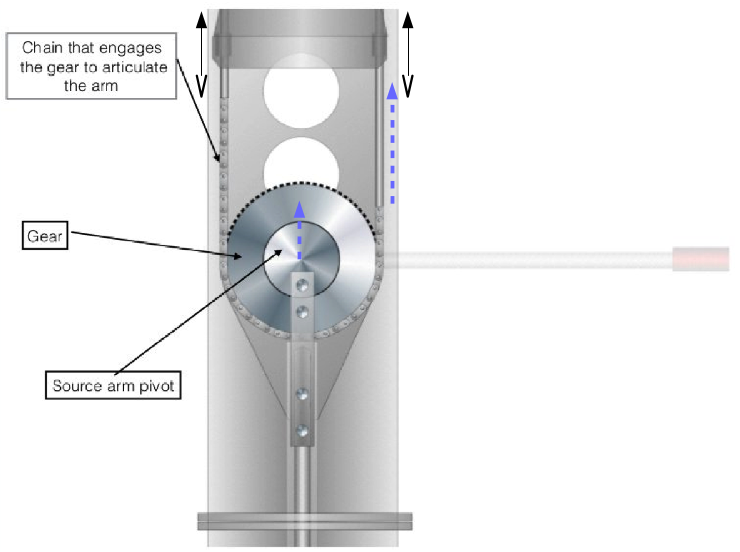
\includegraphics[width=0.48\textwidth]{Figures/sourceArmArticulation.png}
  \caption{\textit{top}: Inside view of the drive mechanism's components seen from the top of CALIS. The stepper motor inside the motor housing drives both cable spools concurrently, thereby lowering the calibration device into the \lsv. An absolute encoder provides the current position of the deployment device. The hand wheel on the left is connected to the left spool only (\textit{bottom left}). When engaged, it drives the gear to transfer the rotation of the articulation wheel into a rotation of the source arm (\textit{bottom right}). The chain has a guard rail, not shown in the drawing, that ensures that the chain can never come off the gear.}
  \label{fig:sourceArmRotation}
\end{figure} 

The stepper motor moves both cable spools concurrently and sends the deployment device into the \lsv. An absolute encoder monitors its current position, even in the absence of power. The stepper motor is controlled via a simple graphical LabVIEW interface, run on a dedicated laptop, in which the current z-position is shown and a target z-position can be provided by the operator. Z-positions are given in motor step counts, an arbitrary unit which has been calibrated outside CRH in meters (Fig.~\ref{fig:z_test}) and relative to the TPC using the t-drift distribution of calibration data (Fig.~\ref{fig:SourcePosition}, p.~\pageref{fig:SourcePosition}).

\begin{figure}[htbp]
 \centering
 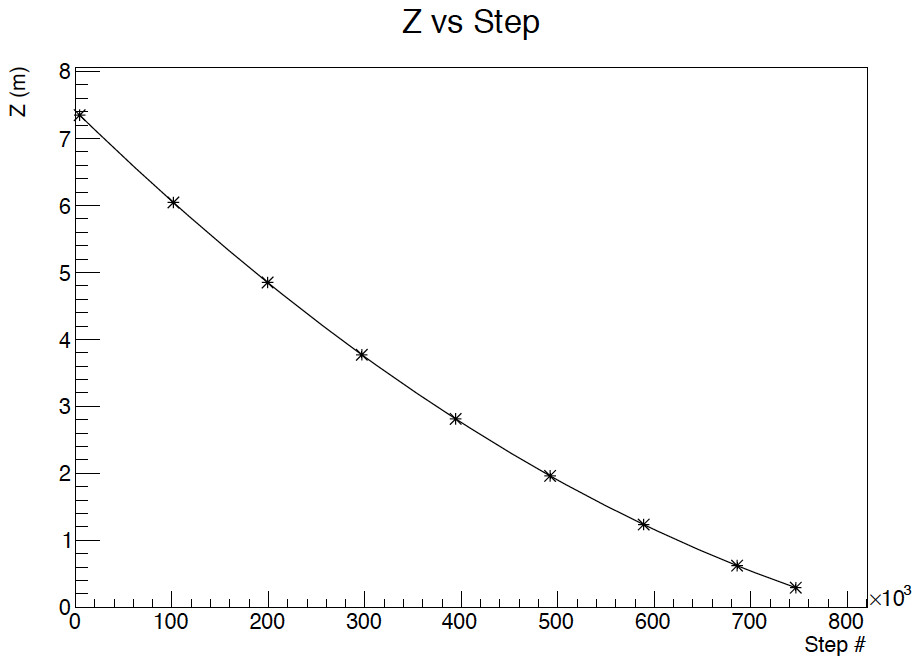
\includegraphics[width=0.65\textwidth]{Figures/Z_positioning_test}
 \caption{Plot of the z position of the deployment device versus the step position of the motor. The non-linear correspondence between the number of steps and the length of cable deployed arises as follows: As the cable winds around the spool, the winding radius changes, increasing as the pig is lifted and decreasing as it is lowered. A motor step count corresponds to a fixed angular distance \textit{d$\theta$}, yet the amount of cable deployed during this motor step count is \textit{winding radius $\cdot$ d$\theta$}. As the winding radius changes as a function of z position, the fraction of deployed cable per motor step count changes.}
 \label{fig:z_test}
\end{figure}

Articulation of the arm is done manually via the articulation wheel. This affects only the cable spool close to the articulation wheel, the left one in Fig.~\ref{fig:sourceArmRotation}, thereby shortening the left cable wrt.~to the right cable and engaging the gear through a chain (Fig.~\ref{fig:sourceArmRotation}). As a result the arm is articulated and the pivot center is lifted. The non-linearity arising from the change in winding radius on the cable spools affects also the amount of rotation required by the hand wheel for horizontal articulation of the source arm.
The degrees corresponding to a horizontal articulation has been calibrated as a function of cable length deployed prior to installation in CRH.

Articulation and a movement in z-direction are mutually exclusive since the articulation of the arm leads to more wound up cable on the spool close to the articulation wheel wrt.~the other. If then in deployment mode both spools would be rotated simultaneously with the same angular speed, the cable close to the articulation wheel would wind up faster than the other, which would lead to a build up of difference in cable length and the deployment device would only be hanging on one cable. In order to avoid an imbalanced z-movement the arm has to be dearticulated fully before a change in z-position can be initiated. This is enforced by an electric switch preventing z-movement, which is disengaged only when the arm is fully dearticulated. 

%Discussion:
% why no permanent tube?
% To complement studies of nuclear recoils with neutron sources ($^{241}$Am$^{9}$Be and $^{241}$Am$^{13}$C), it is planned to deploy a 

\subsection{Housing \& Scintillator}
\begin{figure}[htbp]
 \centering
 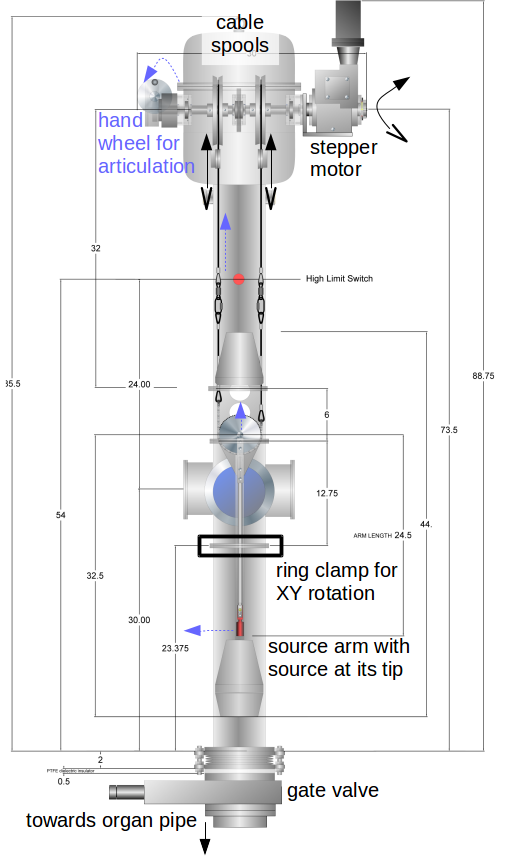
\includegraphics[width=0.68\textwidth]{Figures/CALISDimensions.png}
 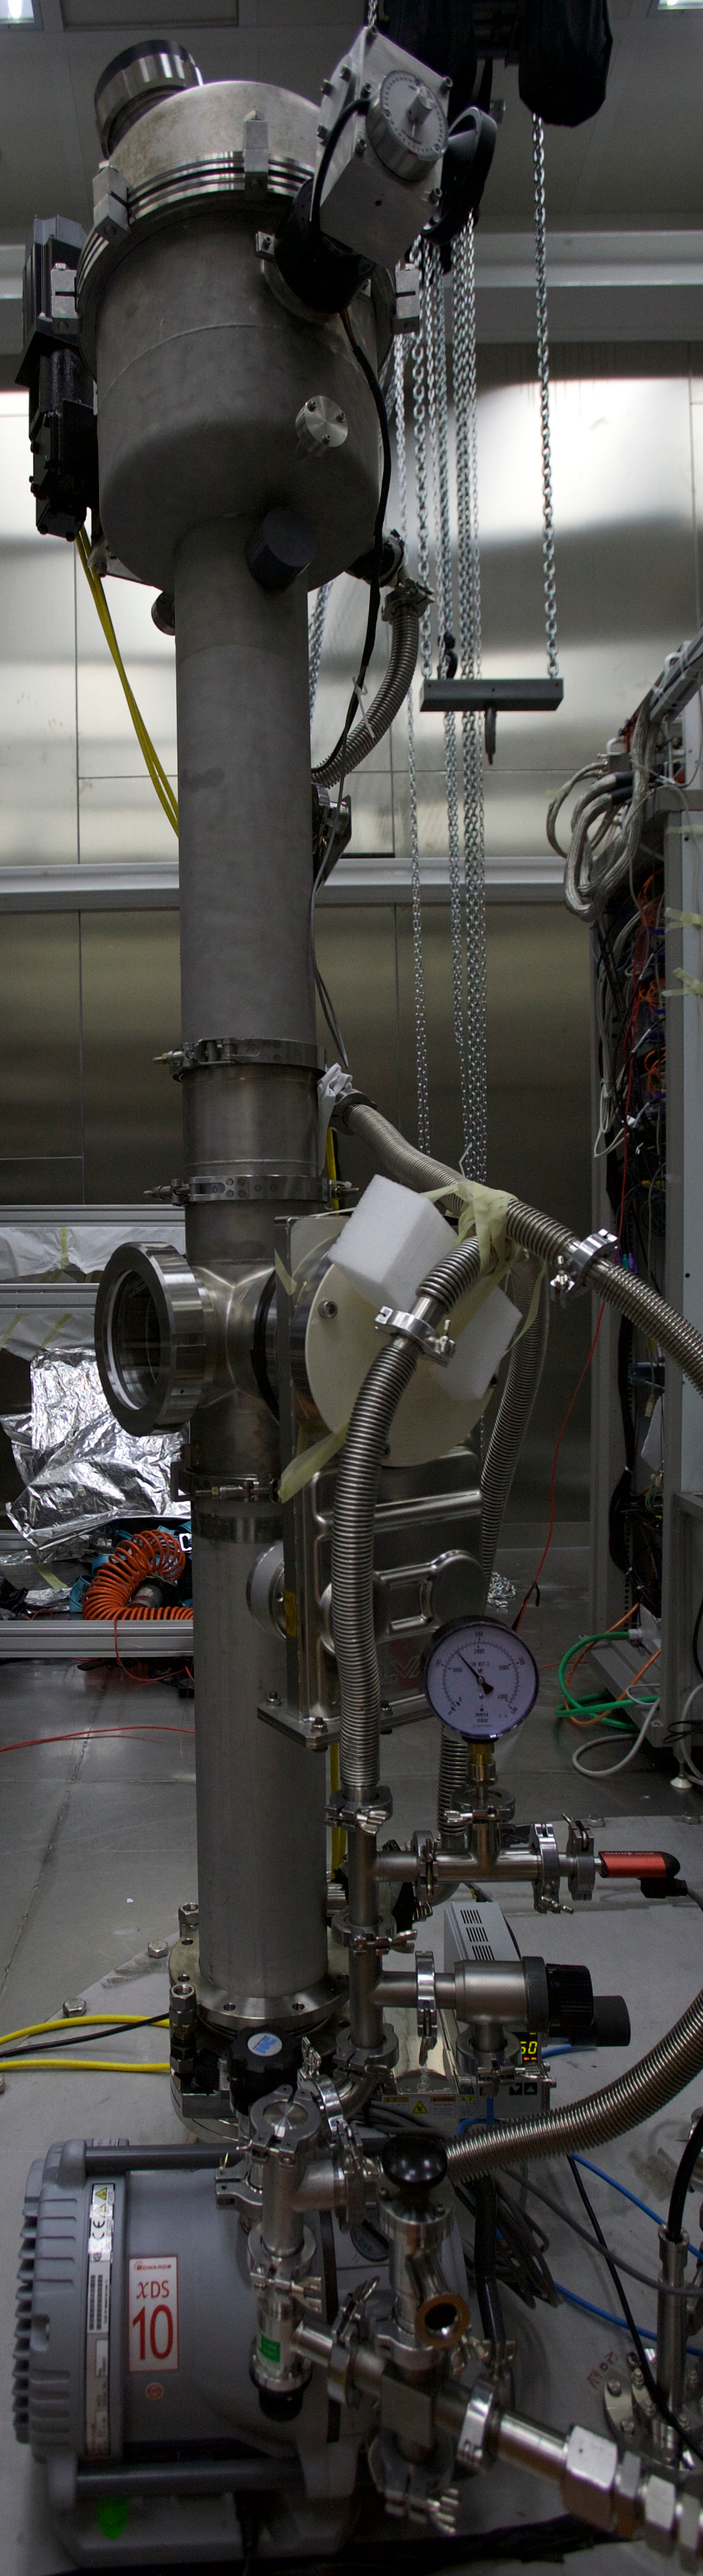
\includegraphics[width=0.30\textwidth]{Figures/CALIS_overview_IMG_3763.jpg}
 \caption{Mechanical drawing of CALIS showing the housing and the deployment device. Dimensions are in inches. (The total height of 88.75 inches corresponds to 225.425 cm.) The two modes of operation are illustrated: In order to move the deployment device down into the LSV or back up the stepper motor moves both cable spools simultaneously. \textcolor{blue}{In order to articulate, the articulation wheel is rotated manually, which affects only the left spool, thereby shortening the left cable wrt.~to the right cable thereby articulating the arm and lifting the pivot center.} The amount of lifting and the amount of rotations until a horizontal articulation is reached has been calibrated prior to installation in CRH (Sec.~\ref{sec:Testing:LNGS})\label{fig:CALISDimensions}\label{fig:CALISMechanism}\label{fig:gearDrawing}
}
\end{figure}

Besides providing mechanical support for the deployment device via the cable spools, the housing is the important interface between CRH and the LSV, through which sources are exchanged, while protecting the liquid scintillator and avoiding human contact with even traces of liquid scintillator vapor at all times (Fig.~\ref{fig:CALISMechanism}). It plays the same role as a glove box for other calibration systems with a narrower foot print inside CRH. The liquid scintillator is a mixture of PC and TMB\footnote{The concentration of TMB has varied during campaigns (see Sec.~\ref{sec:CalibCampaigns}).} with the wavelength shifter PPO\cite{vetoPaper}. It may not get exposed to oxygen or water as is present in normal clean room air and also contamination with $^{222}$Rn and its long-lived radioactive daughters has to be avoided. 
Starting at the gate valve inside the clean room CRH on which CALIS has been installed, a teflon disk allows to electrically isolate CALIS from ground, even though during normal operations the CALIS housing is also connected to ground. A tripod with a bellow has been used to vertically align the housing right after installation on the gate valve. The bellow is connected to a 23.375" long cylindrical stainless steel enclosure pipe. It has the same diameter as the organ pipe (6'') and is connected with the view port by a ring clamp, which plays a critical role in XY rotations (see Sec.~\ref{sec:XYrotation}). The view port can be opened for handling the source arm and exchanging sources. Everything above the ring clamp forms the upper assembly. It features a stainless steel cylindrical enclosure that houses the cable drive mechanism, including the cable spools the stepper motor and the articulation mechanism already described in Sec.~\ref{sec:DeploymentArticulation}. 

\subsubsection*{Vacuum evacuation (flushing) and nitrogen purging}
One of the most important safety features of this system is making sure that the TMB and PC residue on the device are extracted from CALIS prior to opening access ports to exchange source or arms. This is  important for safe working level of the operators as well as for the scintillator and radiopurity. 

After the insertion of the source arm and closure of the view port the inside of the CALIS housing is filled with normal air, that is dangerous to the scintillator. A sequence of several system evacuation and nitrogen purges reduce the fraction of air including its contaminants (water vapor, oxygen, radioactivity) to negligible levels. Only after this sequence the gate valve is opened and the deployment device is introduced into the LSV. Evacuation is achieved with a vacuum pump and dedicated nitrogen and vent lines (Fig.~\ref{fig:flushing_purging}).

This can be addressed through a sequence of system evacuation and nitrogen purge, while the gate . To accelerate the removal of the TMB in the scintillator fluid residue that is left after a deployment, CALIS will undergo an evacuation with a vacuum pump. By lowering the pressure inside of CALIS below the vapor pressure of the TMB, it will cause the TMB to outgas and be removed through the vent line of the vacuum pump. An additional step to remove the TMB is to purge using N$_{2}$.  We will need to limit the potential flow rate of the nitrogen to ensure that an ODH (Oxygen Deficiency Hazard) condition is avoided in CRH.  Only once this is accomplished, will the view port be allowed to be opened and the source handled.     
 
\begin{figure}[htbp]
 \centering
  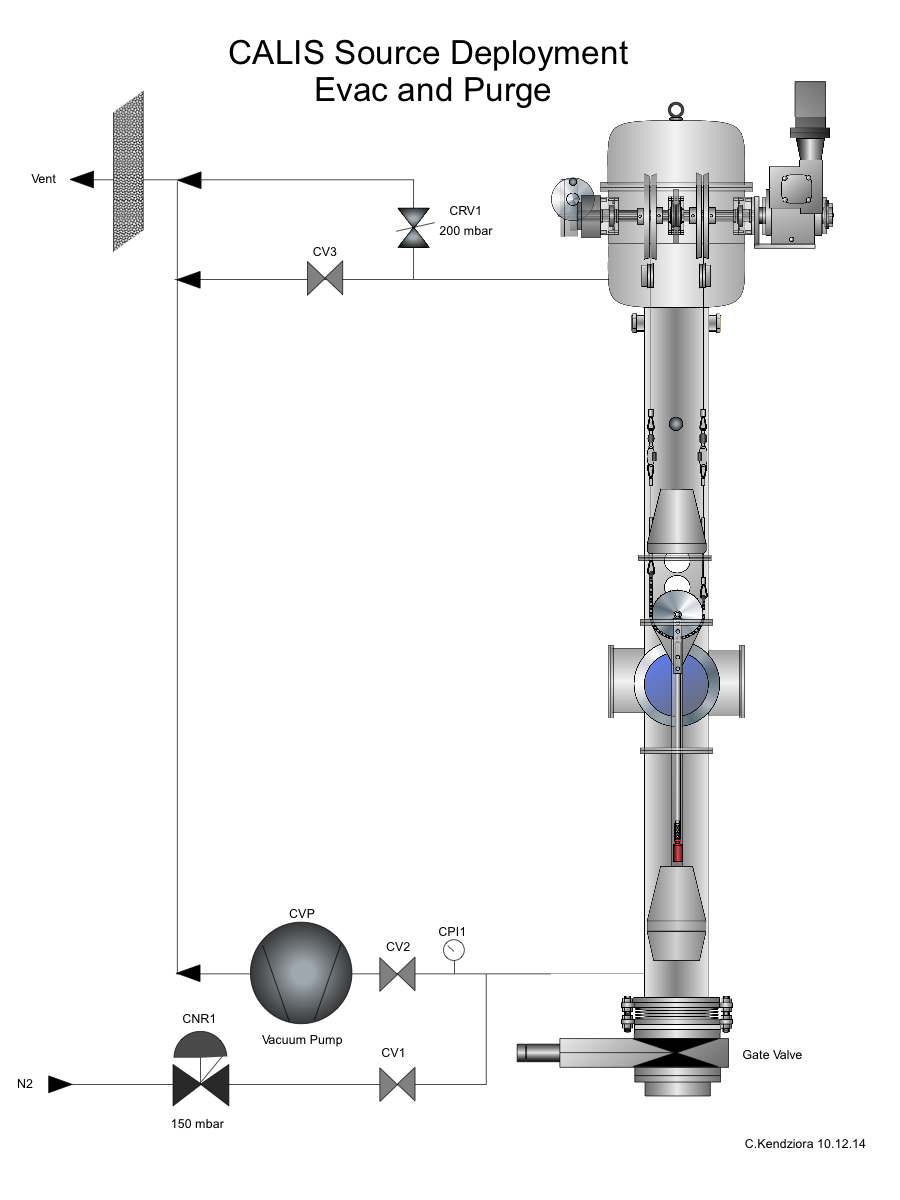
\includegraphics[width=0.73\textwidth]{Figures/GasSystem.png}
  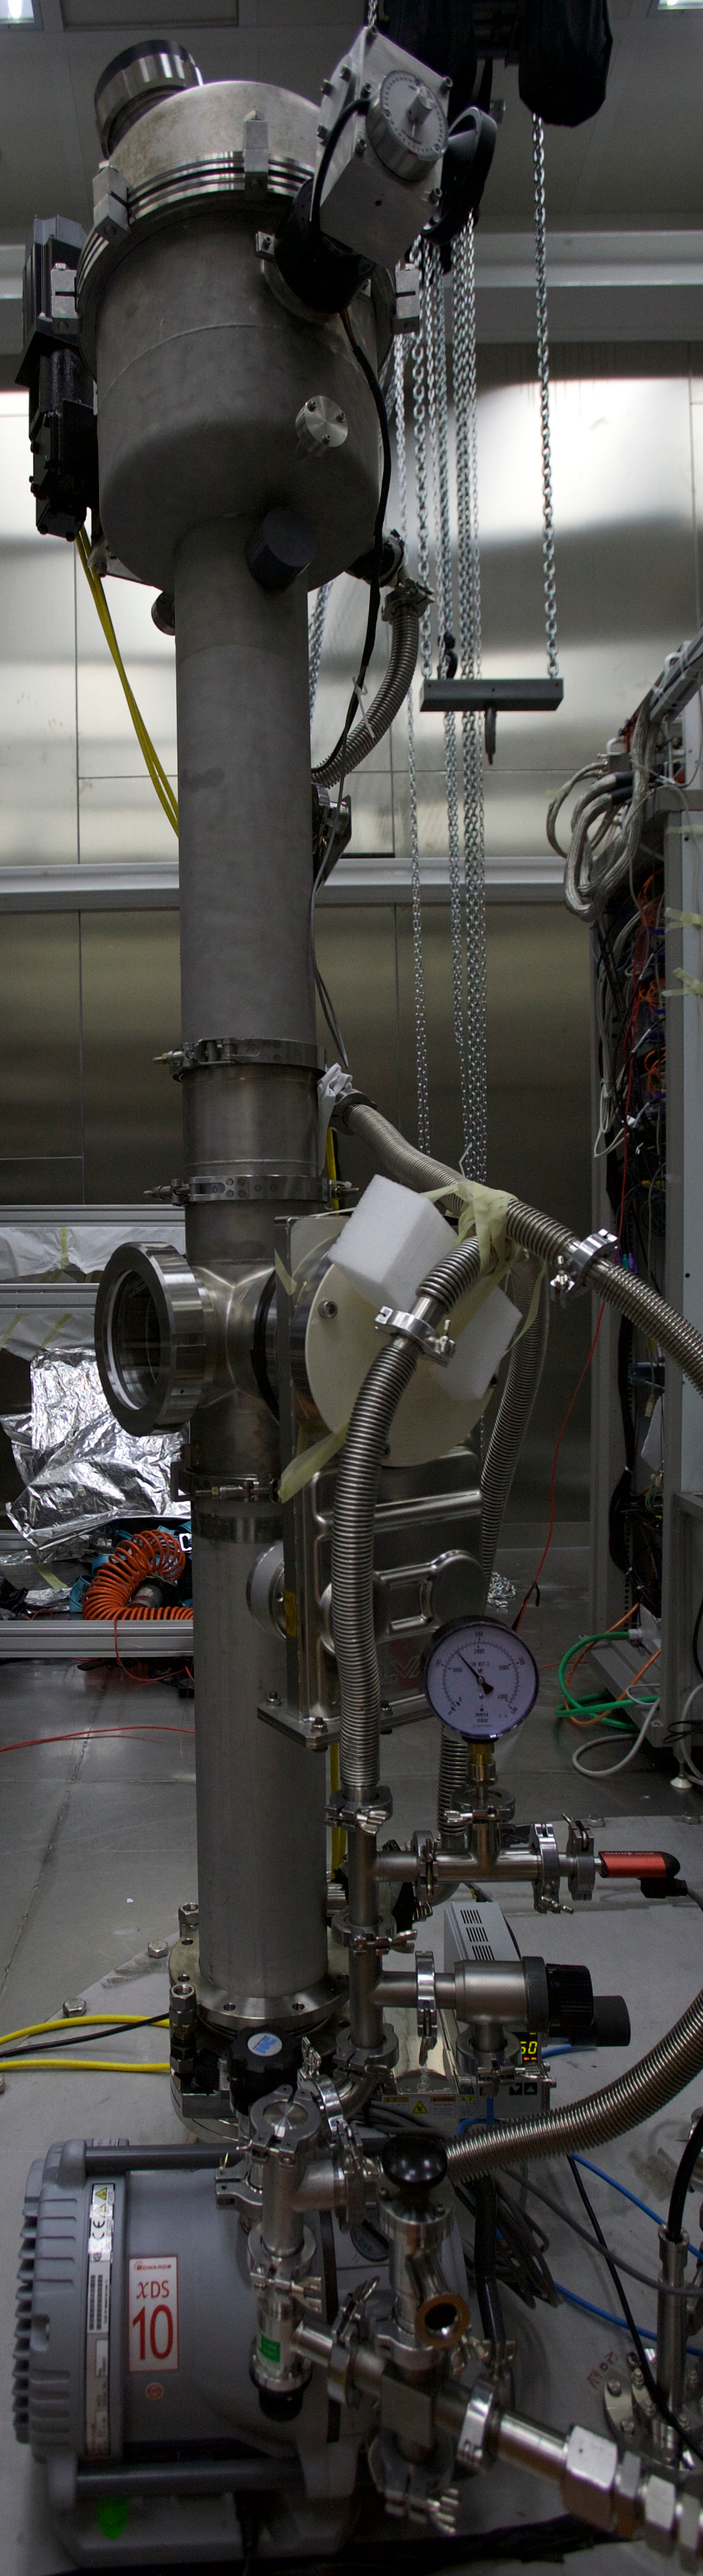
\includegraphics[width=0.25\textwidth]{Figures/CALIS_overview_IMG_3763.JPG}
  \caption{flushing and nitrogen purging system.}
  \label{fig:flushing_purging}
\end{figure}

Vacuum and nitrogen pressurization systems have been developed \ref{sec:N2_pressure_system}.

\subsubsection{Deployment device}
The pig (Fig. \ref{fig:sourcePod_arrows}) contains the support structure for the arm which holds the source at its end.  This piece is equipped with tapered cones on the top and bottom that ensure that the ends do not get snagged on inner edges of the organ pipe as it is moving up and down. It is attached to the housing by two cables.  Swivel hooks are employed in the attachment of the cables to the pig that allow the cables to move freely and not get tangled. 
There are two weights built into the device, one cylindrical in the conical cap above the rotation gear mechanism and one inside the cones at the bottom end of the device. Both help to minimize any lateral motion or oscillations during deployment and articulation and dearticulation especially. It also ensures smooth motion of the deployment device into the organ pipe and back to the home position inside the housing.

\subsubsection{Source holder and arms}
A source arm and the source holder are attached to the articulation gear (Fig.~\ref{fig:SourceHolder}). Different arm lengths have been prepared with a maximum arm length of 62 cm, the arm length thereby being measured from the pivot point of the rotation gear to the tip of the source holder. This arm length allows the source to be placed in immediate contact with the cryostat (Fig.~\ref{fig:CALIS_photos}, right), as the center axis of the organ pipe is 81 cm from the TPC center and the cryostat has an outer radius of 32 cm. The 62 cm arm was used for most of the deployments in the past calibration campaigns (Sec.~\ref{sec:CalibCampaign}). Inside the source holder the radioactive source is placed, pressed to the tip and held in place via a spring during deployment, articulation and dearticulation. The source holder is sealed such that no liquid scintillator can enter during the deployment. This has also been verified during each source extraction, that no liquid was found on the inside.

\begin{figure}[htbp]
 \centering
  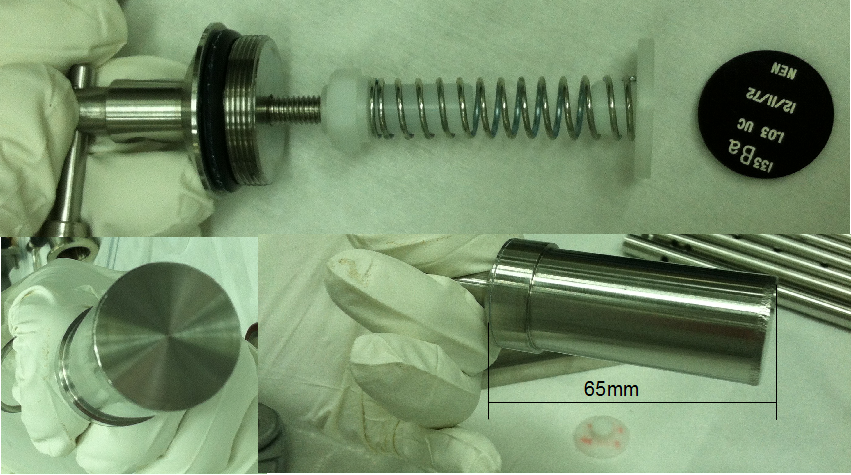
\includegraphics[width=0.7\textwidth]{Figures/SourceHolder.png}
  \caption{Source holder that connects to an arm and to the articulation gear of the deployment device. The source, here a $^{133}$Ba source is pressed to the tip of the source holder via a spring.}
  \label{fig:SourceHolder}
\end{figure}